% !TEX program = xelatex

\documentclass[twocolumn,11pt]{ctexart}

\usepackage[legalpaper, left = 2cm, right = 2cm]{geometry}
%\usepackage[a3paper, total={6in, 8in}]{geometry}





%\usepackage[UTF8]{ctex}

\usepackage{graphicx}
\usepackage{hyperref}
\usepackage{amsmath,amssymb}
\usepackage{algorithm}
%\usepackage{algorithmicx}
\usepackage{algpseudocode}
\usepackage{subcaption}
\usepackage{booktabs}

%\usepackage{multicol}
\usepackage{lipsum}

\newcommand\norm[1]{\left\lVert#1\right\rVert}


\graphicspath{{images/}}


\title{自动化Sprite sheet的生成}
\author{卓越羿 118106010639}
\date{2018}


\begin{document}

\maketitle


\begin{abstract}
    传统2d游戏严重依赖spritesheet(即sprite,如场景中的角色或物体的各种姿态的“差分图像”)生成动画,尽管
    现在有一些基于绑骨的动画更加灵活(如Fire emblem heros的动画),但是要达到精细的效果也十分困难。而如果
    spritesheet能够按照目的自动生成,就能同时到达两者的好处。故本文探索要传统图形方法,传统机器学习方法与
    深度学习方法自动生成spritesheet。分别使用了Delaunay三角形分割映射,正态建模域CycleGAN及其变体实现。
\end{abstract}

\section{概论}

Sprite 是一种游戏或图形应用中2d动画逻辑对象,SpriteSheet则是它的图像素材,
如图 \ref{fig:highpriest} 所示是RPGMaker的一个spritesheet的一部分,表示了
人物的四个方向的行走动作,共3帧。这种像素图在如图所示的小规模时尚易于绘制,
但精细的要求往往使得一个动作就有十几帧高分辨率图像,使得2d的sprite的制作
成本甚至还高于3d,这导致了所谓的3d渲染成2d的技术,不过这种技术对于一些并不
那么符合透视原理的设计并不适合。


\begin{figure}[htb]
    \centering
    
\includegraphics[width=0.3\linewidth]{H.png}
    \caption{Spritesheet例子}
    \label{fig:highpriest}
\end{figure}

另一种2d的技术要求将组件进行分割,然后在组件上再施加旋转缩放位移等表示动画,
如果sprite的动画真就是这些仿射变换可以表示的倒是十分高效,但是若不能则
表现力略逊一筹,或者会为了精细调整引入过多的骨骼,似乎并不比spritesheet高效,
如图\ref{fig:bones}  \cite{zhihu2d}
所示。

\begin{figure}[htb]
    \centering
    \begin{subfigure}[b]{0.4\linewidth}
      
\includegraphics[width=\linewidth]{witch.jpg}
      \caption{sprite}
    \end{subfigure}
    \begin{subfigure}[b]{0.4\linewidth}
      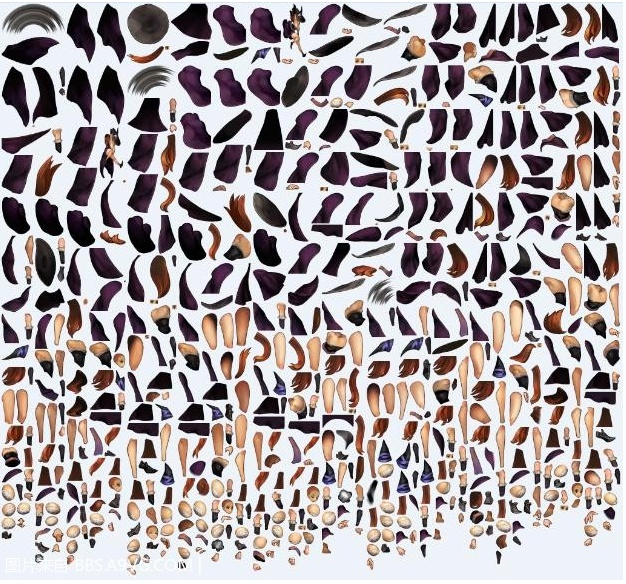
\includegraphics[width=\linewidth]{witch_c.jpg}
      \caption{大量组件}
    \end{subfigure}
    \caption{精细的骨骼动画}
    \label{fig:bones}
\end{figure}

从静态单个图片或几个类似的图片中生成动画的技术有e-mote和live2d,相关
作品有有名的nekopara等,它们主要利用一些变形场之类的方法使得角色可以
做出变动不那么大的“动作”,见图 \ref{fig:miku} 
\footnote{基本就是并不自然的晃来晃去。也许它们唯一
的用处就是让角色有“动”的感觉,不幸的是动图和视频并不能包含在文章中展示这个}
,效果一般来说比较“僵硬”,使得可以一眼看出来是这类技术做出来的。

\begin{figure}[htb]
    \centering
    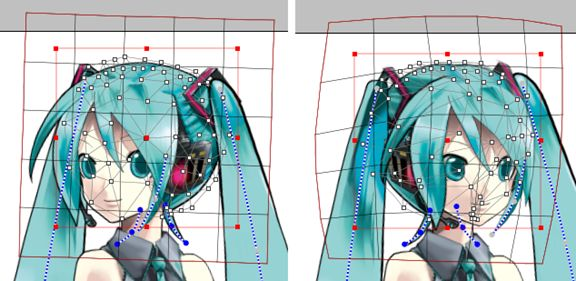
\includegraphics[width=0.7\linewidth]{miku.jpg}
    \caption{变形场}
    \label{fig:miku}
\end{figure}

\section{传统图形法}

\subsection{Delaunay三角形分割映射}

参考图 \ref{fig:highpriest} ,我们可以考虑参考所想要生成的样式直接生成某种模板,然后从原图上将“对应”的纹理直接warp过去,
\cite{swapface}用了类似的方法实现了特朗普,希拉里,克鲁茨\footnote{当时美国共和党竞选者之一}的换脸,效果如图 
\ref{fig:presid}所示。

\begin{figure}[htb]
    \centering
    \begin{subfigure}[b]{0.7\linewidth}
        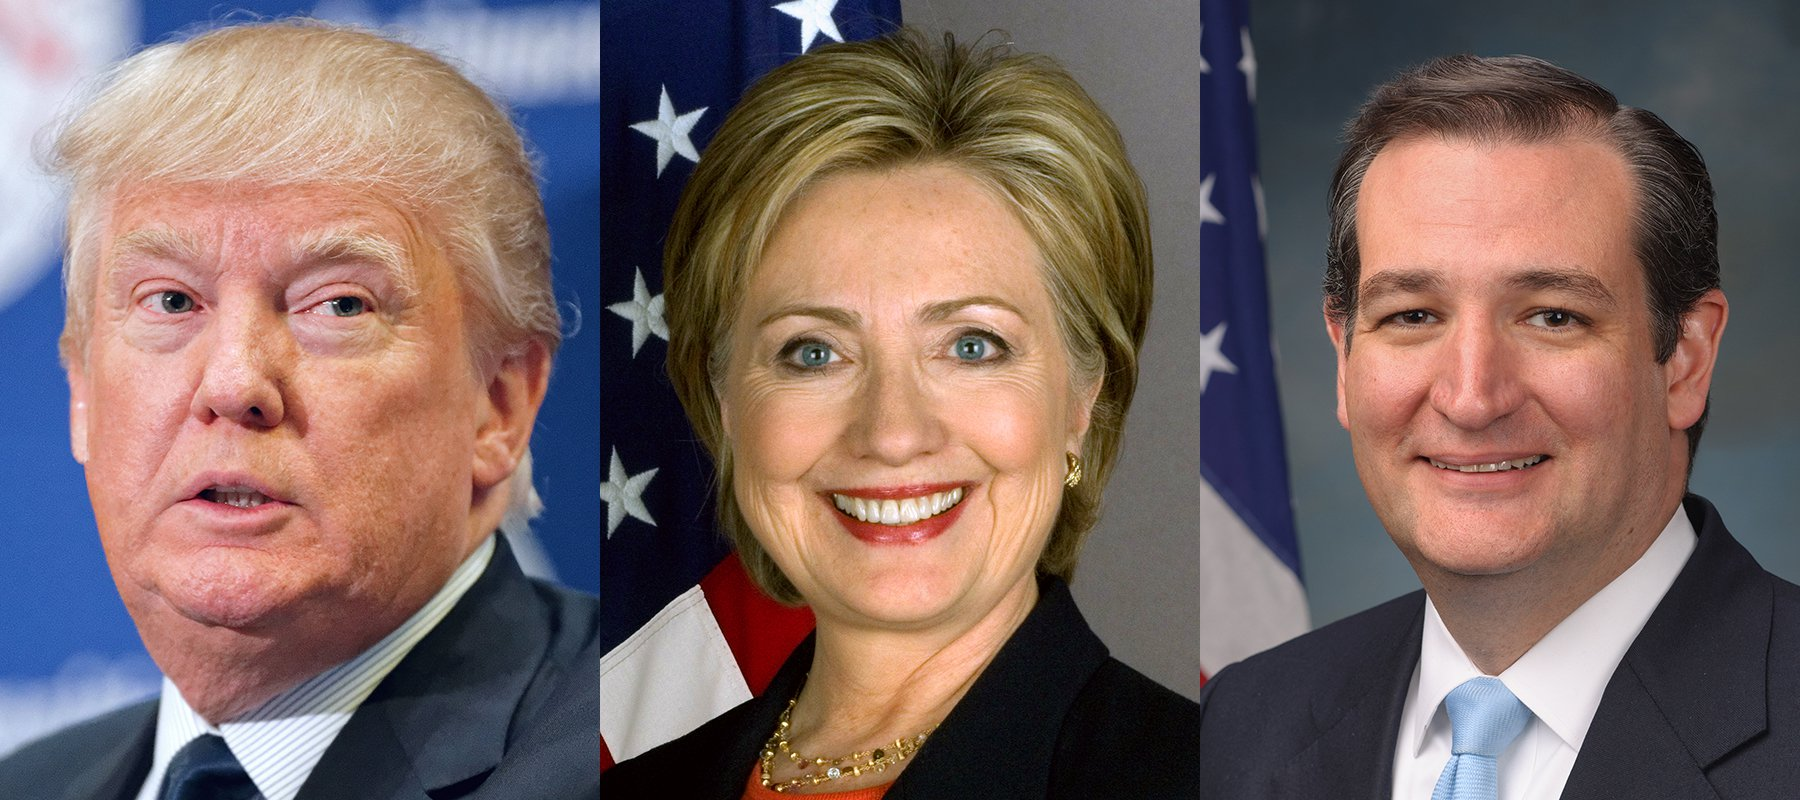
\includegraphics[width=\linewidth]{presidential-original.jpg}
        \caption{原图}
      \end{subfigure}
      \begin{subfigure}[b]{0.7\linewidth}
        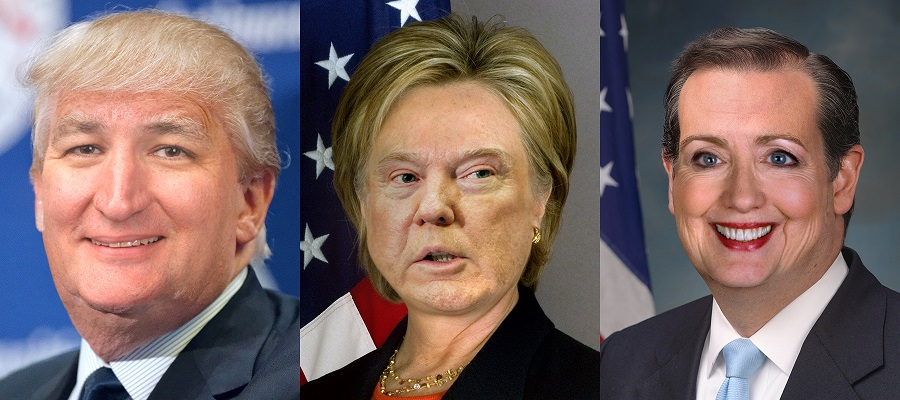
\includegraphics[width=\linewidth]{presidential-swap.jpg}
        \caption{换脸结果}
      \end{subfigure}
      \caption{三个蹩脚竞选人的换脸}
      \label{fig:presid}
\end{figure}

我所用的算法可描述为 算法\ref{alg:delwarp},运行此算法除了两个输入图片外还需要一些关键点,由那些经典的关键点算法得到或者手动标注。
如在\cite{swapface}中它的关键点一部分是用dlib实现的算法\cite{viola2001rapid}其得到的脸部的68个landmarks。
但他为了效果好看起见还补充了12个点。

\begin{algorithm}[htb]
    \caption{Delaunay warp}
    \begin{algorithmic}[1]
    \Procedure{Delaunay warp}{img1, img2, points1, points2}
        \State out $\gets$ img2
        \State dt $\gets$ 计算被points对应的的Delaunay三角形
        \For{t in dt}
            \State t1 $\gets$ points1[t]
            \State t2 $\gets$ points2[t]
            \State trans $\gets$ 拟合t1到t2的仿射变换
            \State out $\gets$ trans(out, img1, trans) 
        \EndFor
        \State \textbf{return} out
    \EndProcedure
    \end{algorithmic}
    \label{alg:delwarp}
\end{algorithm}

Delaunay三角划分就是取所有点的可能的边中的一些这样的边——它使得它围成的多边形只有三角形(自然也没有交点),
且这些三角形的外接圆不包含其他顶点\cite{Delaunay} \cite{delaunay1934sphere}。
这使得它倾向于产生锐角(均匀)三角形,这正是warp所需要的。

与\cite{swapface}的算法不同的是它求了关键点的凸包并只取构成凸包的顶点(从而68个点中大多数其实没起作用),并在最后运用了
Poisson Image Editing \cite{perez2003poisson} 的技术进行了平滑。它求凸包很大程度上是为了最后运用Poisson Image Editing,但是我的目标域是
透明的,并不需要平滑,所以可以多取一些Delaunay三角形使得纹理分割更细致一些。

将长者和RPGMaker中的国王的spritesheet的一帧运行此算法,关键点由手工标注,如图 \ref{fig:map} 所示。
warp迭代过程如图 \ref{fig:elder2king} 所示。这个算法当然也可以反过来进行,将国王warp为长者的迭代
过程如图 \ref{fig:king2elder}所示。 

\begin{figure}[htb]
    \centering
    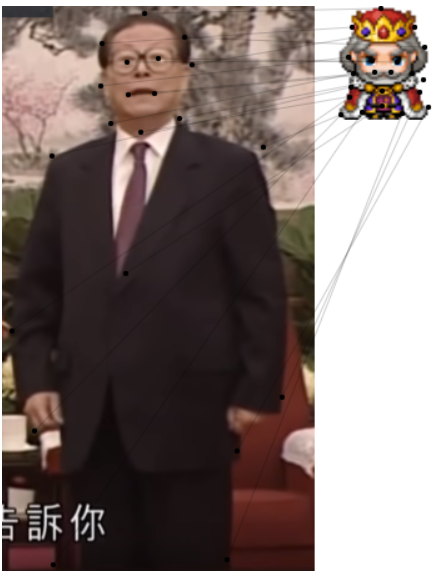
\includegraphics[width=0.5\linewidth]{map.png}
    \caption{长者与国王的关键点对应}
    \label{fig:map}
\end{figure}

\begin{figure}[htb]
    
\includegraphics[width=\linewidth]{tri_elder2king.png}
    \caption{将长者warp为国王}
    \label{fig:elder2king}
\end{figure}

\begin{figure}[htb]
    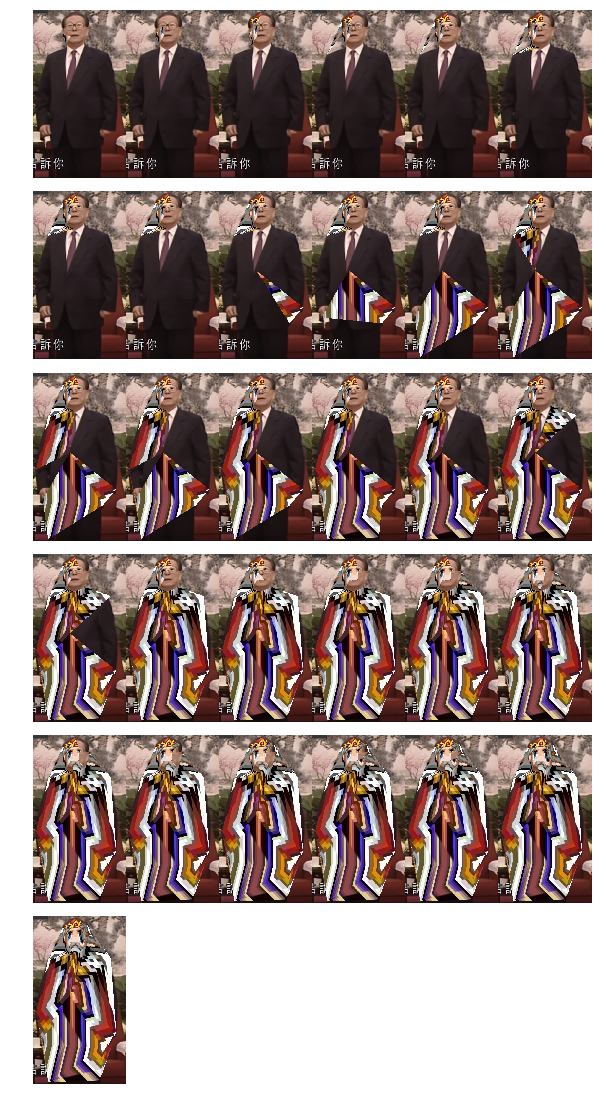
\includegraphics[width=\linewidth]{tri_king2elder.png}
    \caption{将国王warp为长者}
    \label{fig:king2elder}
\end{figure}

由于国王的头朝向偏下,而长者偏上,所以导致长者的头部的极度扭曲,正如\cite{swapface}中所指出的那样它无法处理
pose的转化问题,毕竟它只不过是尽可能把纹理映射过去罢了。更精细的划分,正如变形场\ref{fig:miku}所展示的那样,
一定程度上可以缓解这个问题,但看上去并不本质,也许分离出pose与纹理,甚至反推出背后的3d模型才是解决问题的
正确方式,正如\cite{yingzhen2018disentangled}的方法一样,不过那是深度学习的,只能放在后面根据要求。


\section{传统机器学习方法}

狭义上传统机器学习能用来生成的方法似乎不多,不过广义的来看线性回归$Y_i = X_i \beta + \epsilon_i$
甚至都可以用来生成,我们只需要根据$\epsilon \sim N(0,\sigma)$生成一段噪声$\epsilon_i$,把它代进去
就可以生成某种有规律的输出。正如白噪声通过一个成型滤波器称为正相关的,类似随机游走的时间序列一样,
如图\ref{fig:shaping}所示,是白噪声 $x[n] \sim N(0,1)$ 与 $y[n] = x[n] + x[n-1] + x[n-2] +x[n-3]$的
对比。而这与GAN隐式的拟合一个映射表示一个分布有异曲同工之妙。

\begin{figure}[htb]
    \centering
    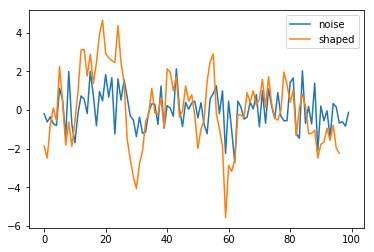
\includegraphics[width=0.6\linewidth]{shaping.png}
    \caption{成型滤波器}
    \label{fig:shaping}
\end{figure}


\subsection{正态模型}

收集RPGMaker自带的1332个像素图(由图 \ref{fig:highpriest} 那样的图分出12个子图得),拉成向量后求其均值与协方差矩阵
可以得到此类图像分布的多元正态模型,如期望是类似平均脸的东西,如图 \ref{fig:meansd} 所示。 

\begin{figure}[htb]
    \centering
    \begin{subfigure}[b]{0.3\linewidth}
        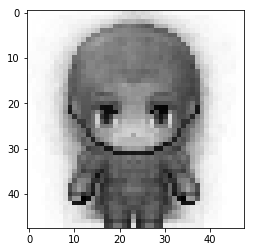
\includegraphics[width=\linewidth]{mean_sprite.png}
        \caption{均值}
      \end{subfigure}
      \begin{subfigure}[b]{0.3\linewidth}
        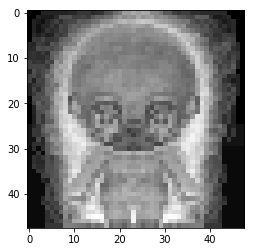
\includegraphics[width=\linewidth]{sd_sprtie.png}
        \caption{标准差}
      \end{subfigure}
      \caption{sprite分布特征}
      \label{fig:meansd}
\end{figure}

形式地,模型为:

$$
X \sim N(\mu, \Sigma) \quad X \in R^d
$$

其中$d=48^2=2304$,为拉长向量的维度。

在变分推断对$\Sigma$的设定中会用到meanfield(约束只有对角元素非0)或fullrank(所有元素可任取,当然要保持半正定)等,
统计还专门有所谓“协方差结构”理论来限制参数数量以免自由度不足,但同时又添加必要的参数考虑一些特定的相关,如三对角矩阵
之类的。
不过这里由$2304^2 = 5308416$个参数构成的fullrank式协方差矩阵还能接受,毕竟在深度学习里这也就一层的参数量。

\subsubsection{直接采样}

无论如何设定,多元正态分布可以下式直接采样,协方差矩阵$\Sigma$是实对称矩阵,
所以有cholesky分解\footnote{实际计算用的svd分解算的},$\Sigma = LL^T$,
从而可通过下式生成$N(\mu,\Sigma)$型随机变量,根据$AX+b \sim N(\mu_X + b, A\Sigma_XA^T)$:

\begin{align*}
    X &\sim N(0, I) \\
    Y &= L X + \mu \sim N(0+\mu,LIL^T) = N(\mu, \Sigma)
\end{align*}

采样中主要计算cholesky分解比较费时。meanfield与fullrank的采样结果比较如图 \ref{fig:meanfieldfullrank} 所示。
可以看出fullrank的结果比meanfield的平滑得多,没那么多谜之噪声,这显然是考虑到像素间相关的功劳。

\begin{figure}[htb]
    \centering
    \begin{subfigure}[b]{0.7\linewidth}
        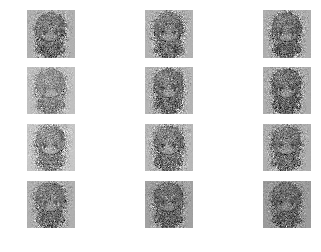
\includegraphics[width=\linewidth]{meanfield.png}
        \caption{meanfield}
      \end{subfigure}
      \begin{subfigure}[b]{0.7\linewidth}
        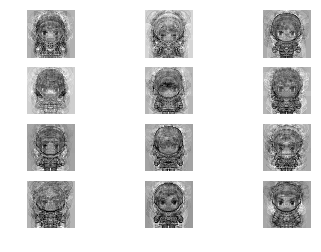
\includegraphics[width=\linewidth]{fullrank.png}
        \caption{fullrank}
      \end{subfigure}
      \caption{正态模型直接采样}
      \label{fig:meanfieldfullrank}
\end{figure}

\subsubsection{条件采样}

利用多元正态分布的条件分布关系:

\begin{align*}
(x_1 \, x_2) &\sim N((\mu_1,\mu_2),\Sigma) \\ 
x_1 \mid x_2 = a &\sim N(\bar{\mu},\bar{\Sigma}) \\
\bar{\mu} &= \mu_1 + \Sigma_{12}\Sigma^{-1}_{22}(a - \mu_2) \\
\bar{\Sigma} &= \Sigma_{11} - \Sigma_{12}\Sigma_{22}^{-1}\Sigma_{21}
\end{align*}

可以进行条件采样,下面将6个没有列入训练集的样本分别把上半部下半部分左半部分右半部分遮住,
用没遮住的另一边去计算其条件分布进行采样。不过实际计算中协方差矩阵四个分块矩阵都是数值奇异的,所以要计算逆的地方
均计算了伪逆。结果的变异不够,实际发现边缘协方差矩阵$\bar{\Sigma}$的广义方差(取$trace$的话)非常小,
其中一个只有$2.3047376846740273e-08$的程度,而原来四个协方差矩阵的trace则为
$3450960.26, 162045.6, 162045.66, 4577188.87$
考虑到利用SVD分解可以将维度从降到2304降到150而数值上无法区分出来。强行引入$2304/2=1152$个约束似乎使得条件分布
的变异太小了\footnote{尽管因为用伪逆取代了逆,这个定义本来就是病态的},所以每个设定下只取了一个样本显示出来,
如图  \ref{fig:normcond1}所示。如果是训练集的样本的话会完全重建,完全不辜负它几百万个参数,
如图 \ref{fig:normcond2}所示。

\begin{figure}[htb]
  \centering
  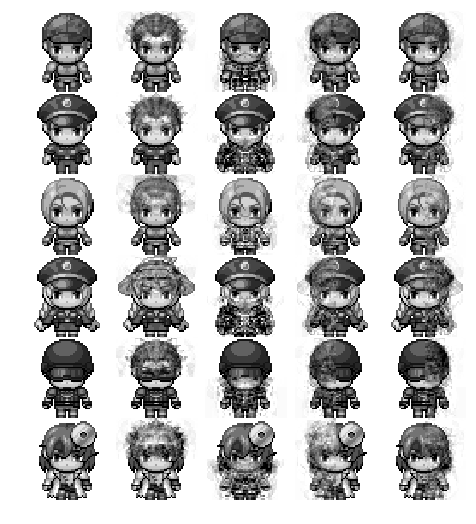
\includegraphics[width=0.6\linewidth]{normal_conditional_sample.png}
  \caption{正态条件采样,测试集}
  \label{fig:normcond1}
\end{figure}

\begin{figure}[htb]
  \centering
  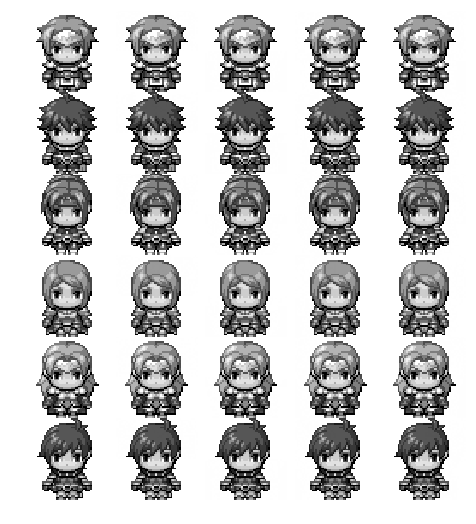
\includegraphics[width=0.6\linewidth]{normal_conditional_sample2.png}
  \caption{正态条件采样,训练集}
  \label{fig:normcond2}
\end{figure}

条件推断会比较有用,因为很多图只有人物的上半身而没有下半身,所以我们可以让模型只取上半身去“脑补”出对应的下半身,
图\ref{fig:normalreal} 显示了来自真实图像(参考 \ref{fig:hp2sprite}) 与我手画的火柴人的推断结果。
毫不奇怪的结果十分猎奇,果然这种本质硬模板的方法至多在同分布的情况下用用。

\begin{figure}[htb]
  \centering
    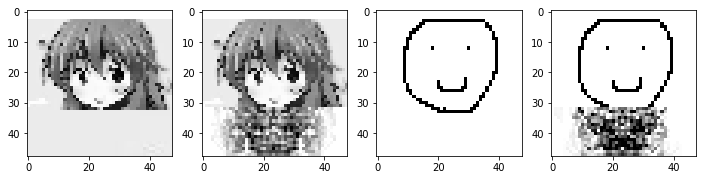
\includegraphics[width=\linewidth]{normal_real_test.png}
    \caption{HP和火柴人的正态模型条件推断}
    \label{fig:normalreal}
\end{figure}


某种意义上说正态模型和它的推断,如delta方法等与神经网络那一套有点像,如全连接层的多变量的映射关系只考虑线性部分,
相当于一个一阶泰勒展开。多元正态分布刻画相关也只考虑二阶矩。神经网络刻画更复杂的关系要叠加非线性层,多元正态
也可以引入混合模型与层次模型。神经网络可以逼近任意函数,中心极限定理也保证很多统计量渐进正态分布。(完 全 一 致)

\section{深度学习方法}

\subsection{CycleGAN}

CycleGAN \cite{zhu2017unpaired} 提供了一种无监督的将两个图像域中的图像转换的方法,如将马换成斑马或者狗变猫等。

它由四个网络构成,GA,GB,DA,DB,GA试图将A域图片转成B域图片,GB则试图将B域图片转为A域图片。DA,DB则鉴别一个图片
是来自真实分布$p_{data}(x)$还是来自由GA,GB定义的隐式分布$GA(y) \quad y \sim p_{data}(y)$。

收到要写这个大作业后我首先想到的方法就是这个,不幸的是因为我个人电脑只有GTX1050ti,
其4g显存运行不动原论文提到的输入规模($256\times256$)。
我的样本的A域是RO中HP各种图,B域是类似 \ref{fig:highpriest} 那样的图,如图 \ref{fig:hp2sprite} 所示,
在不同的架构中B域的sprite图有时会被增大。

\begin{figure}[htb]
    \centering
    \begin{subfigure}[b]{0.3\linewidth}
        
\includegraphics[width=\linewidth]{hp.jpg}
        \caption{A域}
      \end{subfigure}
      \begin{subfigure}[b]{0.3\linewidth}
        
\includegraphics[width=\linewidth]{bigsprite.png}
        \caption{B域}
      \end{subfigure}
      \caption{CycleGAN数据集}
      \label{fig:hp2sprite}
\end{figure}

它的损失设定为:
\begin{align*}
\mathcal{L}(G,D) &= \mathcal{L}_{GAN}(G_A,D_B) \\
                             &+ \mathcal{L}_{GAN}(G_B,D_A) \\
                             &+ \lambda \mathcal{L}_{cyc}(G_A,G_B) + \gamma \mathcal{L}_{iden}(G_A,G_B) \\
  \mathcal{L}_{GAN}(G_X,D_Y) &= \mathbb{E}_{y\sim p_{data}(y)}(\log D_Y(y))  \\
                             &+ \mathbb{E}_{x \sim p_{data}(x)} \log(1-D_Y(G(x)))  \\
  \mathcal{L}_{cyc}(G_A,G_B) &= \mathbb{E}_{x\sim p_{data}(x)} (\norm{G_B(G_A(x)) - x}_1) \\
                             &+ \mathbb{E}_{y\sim p_{data}(y)} (\norm{G_A(G_B(y)) - y}_1) \\
 \mathcal{L}_{iden}(G_A,G_B) &= \mathbb{E}_{y \sim p_{data}(y)}(\norm{G_B(y)-y}_1) \\
                             &+ \mathbb{E}_{x \sim p_{data}(x)}(\norm{G_A(x)-x}_1)
\end{align*}

其中$\mathcal{L}_{GAN}(G_X,D_Y)(X,Y \in \{A,B\})$定义了$A \to B$与$B \to A$的GAN损失,也就是将来自A域样本判成由B域经$G_B$生成的
假A样本与将假A样本判成真A样本均带来损失。这个损失是对$D_A,D_B$来说的。对$G_A,G_B$,可以看作把真实样本判成错的损失拿掉,
因为$G_X$的参数本身也不能控制这个错误,而把把将它生成的错判伪造样本取负,即向鼓励$D_X$错判的方向优化。

循环损失$\mathcal{L}_{cyc}(G_A,G_B)$约束网络应该应当在将一个A域的图由$G_A$变为B域的图后,
再由$G_B$变回来时大致相同。可看成一种正则项,但实际训练时会发现有时由于$D_X$过于强大,主要目标$\mathcal{L}_{GAN}$
在小参数变化下没什么起色,结果算法就一股劲去优化这个循环损失了,反而加剧了GAN训练死亡困境。

恒等映射损失$\mathcal{L}_{iden}$要求B域图片经过$G_A$映射($G_A$本身被要求把$A$域的图片映射到$B$域)应该没有变化。
这个损失在原文\cite{zhu2017unpaired}是个可选的正则项,也有之前提到的问题。另外这个项的引入使得默认了两个域的图像
尺寸一样,而我的问题里两个域的图像尺寸是不一样的,所以我分别用了把两个域的图片转成一样的与改变这个损失的定义的方法。

分类器$D_X$与生成器$G_X$对每个样本各训练一次为一个epoch,有时考虑分类器过于强大也考虑让生成器多训练几个step或者
调大学习率,不过感觉效果不明显。

\subsubsection{实验1}

网络结构与 \cite{zhu2017unpaired}的基线实现完全一致,
其中GA(B)就是resnet\_9blocks的实现,结构为:

c7s1-64,d128,d256,R256,R256,R256,R256,
R256,R256,R256,R256,R256,u128,u64,c7s1-3。

其中c7s1-64指有64个$7\times7$filters,stride为1的卷积层,负责在channel较少时进行大卷积扩大感受野与平滑
。dk(reduce)为k个filters的stride为2的降图像尺寸的卷积层。R256为256个filters的,由\cite{he2016deep}
提出的residual block,具有在不合适的时候关闭自己的能力(即变为恒等映射),以便于大深度训练,虽然这里也称不上多深。
uk(undoreduce)为k个filters,strides为$1/2$的卷积层,即DCGAN \cite{radford2015unsupervised}等用的转置/反卷积层,
负责将图像以一定规律放大一倍,其与升采样1倍再用个类似R256的层“平滑”效果是否有显著差别尚无定论
\footnote{我两年前实现DCGAN时看到这两个方法都有使用}。所有层后均有InstanceNorm-ReLU层。
其中InstanceNorm我之前倒没用过,以前都是BatchNorm,
它们都是面向filters级的标准化,但BatchNorm是把空间维与Batch维都加进来标准化 \cite{ioffe2015batch}:

\begin{align*}
y_{tilm} &= \frac{x_{tilm} - \mu_i}{\sqrt{\sigma_i^2 + \epsilon}} \\
\mu_i &= \frac{1}{HWT}\sum_{t=1}^T\sum_{l=1}^W\sum_{m=1}^H x_{tilm} \\
\sigma_i^2 &= \frac{1}{HWT}\sum_{t=1}^T\sum_{l=1}^W\sum_{m=1}^H (x_{tilm} - \mu_i)^2
\end{align*}

而InstanceNorm \cite{vedaldi2016instance}在各个batch内分别标准化,只用空间维的信息估计“参数”:

\begin{align*}
    y_{tilm} &= \frac{x_{tilm} - \mu_{ti}}{\sqrt{\sigma_{ti}^2 + \epsilon}} \\
    \mu_{ti} &= \frac{1}{HW}\sum_{l=1}^W\sum_{m=1}^H x_{tilm} \\
    \sigma_{ti}^2 &= \frac{1}{HW}\sum_{l=1}^W\sum_{m=1}^H (x_{tilm} - \mu_{ti})^2
\end{align*}

InstanceNorm之所以被使用是因为 \cite{vedaldi2016instance}等一些文章指出它们在风格迁移问题上效果更好。

DA(B)的网络结构也完全一致,也就是 C64-C128-C256-C512 ,其中Ck指 $4\times 4$,k个filters,stirdes为2的卷积层,
各层后均有InstanceNorm-LeakyReLU(斜率为0.2)层,除了C64后没有InstanceNorm外。这个卷积网络的感受野为70,所以
也被称为$70\times 70$ PatchGAN,它的输出是一个不定大小的指明各点对应感受野上的分类概率的feature map,
这个feature map的每个值被都看作与真实标签(来自$p_{data}(y)$还是$G(x) \quad x\sim p_{data}(x)$)形成
一个样本计算损失。

输入从$256 \times 256$改成$64\times64$的以外
(B域图片本身是$48\times 48$的,A域的尺寸不定),这个的A,B域图片使用crop+warp增强。这个我观测了24个epochs结果
后感觉效果不好就停止了训练。最终效果如图 \ref{fig:exp1} 所示(A域原图因为不太合适和谐掉了)。可以看到如果说
$G_A(x) x\in A$还有点形状外,$G_B(y)$就可以说是至多迁移了点纹理罢了。

\begin{figure}[htb]
    \centering
    \begin{subfigure}[b]{0.24\linewidth}
        
\includegraphics[width=\linewidth]{NSFW.png}
        \caption{$x \in A$}
      \end{subfigure}
      \begin{subfigure}[b]{0.24\linewidth}
        
\includegraphics[width=\linewidth]{exp1_fake_B.png}
        \caption{$G_A(x)$}
      \end{subfigure}
      \begin{subfigure}[b]{0.24\linewidth}
        
\includegraphics[width=\linewidth]{exp1_real_B.png}
        \caption{$y \in B$}
      \end{subfigure}
      \begin{subfigure}[b]{0.24\linewidth}
        
\includegraphics[width=\linewidth]{exp1_fake_A.png}
        \caption{$G_B(y)$}
      \end{subfigure}
      \caption{实验1结果}
      \label{fig:exp1}
\end{figure}


\subsubsection{实验2}

实验1之所以之运行了24个epoch就结束了是因为我突然感觉B域不应该使用random crop增强,实验1是看到默认的recale到
短边为286像素的图片,然后取其中的$256 \times 256$的random crop,是AlexNet以来的方法,,所以取了
rescale到100像素,然后取64像素的random crop。不过我觉得我这就是要
让它在特定的区域是白(透明)的,而这个增强似乎并没有带来这个结果,如图\ref{fig:exp1}所示,$G_A(x)$的图似乎有些
靠右的感觉,这并不是我想要的。所以我改成了缩放为短边为64像素后取$64 \times 64$random crop,这只对A域的图片是随机的。

迭代过程可以说大起大落,开始$G_A(x)$基本只是往A域图片上加一些B域图片对比度很强的纹理,将边缘裁剪掉,
如图 \ref{fig:exp2epoch4} 所示。其中$G_{BA}(x)=G_B(G_A(x))$,另一个类似,为了排版好看起见。另外
$G_A(x)$表示$G_A$试图将A域图片变为B域图片的结果,我们的目标是它看起来像个sprite,理想情况下我们的感觉与
$\mathcal{L}_{GAN}$应该是一致的。而$G_B(G_A(x))$表示重建的结果,理想情况是与$x$十分相近,这里对应着
$\mathcal{L}_{cyc}$的L1损失。而$G_B(x)$则表示把一个本来就是A域的图片喂给试图将B域图片转为A域图片的
$G_B$的结果,理想情况也是与A域图片一致。另外对称的四个图片的意思类似不再解释。

\begin{figure}[htb]
    \centering
    \begin{subfigure}[b]{0.23\linewidth}
        
\includegraphics[width=\linewidth]{exp2_epoch004_real_A.png}
        \caption{$x \in A$}
      \end{subfigure}
      \begin{subfigure}[b]{0.23\linewidth}
        
\includegraphics[width=\linewidth]{exp2_epoch004_fake_B.png}
        \caption{$G_A(x)$}
      \end{subfigure}
      \begin{subfigure}[b]{0.23\linewidth}
        
\includegraphics[width=\linewidth]{exp2_epoch004_rec_A.png}
        %\caption{$G_B(G_A(x))$}
        \caption{$G_{BA}(x))$}
      \end{subfigure}
      \begin{subfigure}[b]{0.23\linewidth}
        
\includegraphics[width=\linewidth]{exp2_epoch004_idt_A.png}
        \caption{$G_A(y)$}
      \end{subfigure}
      \begin{subfigure}[b]{0.23\linewidth}
        
\includegraphics[width=\linewidth]{exp2_epoch004_real_B.png}
        \caption{$y \in B$}
      \end{subfigure}
      \begin{subfigure}[b]{0.23\linewidth}
        
\includegraphics[width=\linewidth]{exp2_epoch004_fake_A.png}
        \caption{$G_B(y)$}
      \end{subfigure}
      \begin{subfigure}[b]{0.23\linewidth}
        
\includegraphics[width=\linewidth]{exp2_epoch004_rec_B.png}
        %\caption{$G_A(G_B(y))$}
        \caption{$G_{AB}(y))$}
      \end{subfigure}
      \begin{subfigure}[b]{0.23\linewidth}
        
\includegraphics[width=\linewidth]{exp2_epoch004_idt_B.png}
        \caption{$G_B(x)$}
      \end{subfigure}
      \caption{实验2epoch4的结果}
      \label{fig:exp2epoch4}
\end{figure}

到了epoch 60 见图\ref{fig:exp2epoch60},看上去好像就要成功了,身体的各部分的对应还算正确,虽然形状比较鬼畜。

\begin{figure}[htb]
    \centering
    \begin{subfigure}[b]{0.23\linewidth}
        
\includegraphics[width=\linewidth]{exp2_epoch060_real_A.png}
        \caption{$x \in A$}
      \end{subfigure}
      \begin{subfigure}[b]{0.23\linewidth}
        
\includegraphics[width=\linewidth]{exp2_epoch060_fake_B.png}
        \caption{$G_A(x)$}
      \end{subfigure}
      \begin{subfigure}[b]{0.23\linewidth}
        
\includegraphics[width=\linewidth]{exp2_epoch060_rec_A.png}
        %\caption{$G_B(G_A(x))$}
        \caption{$G_{BA}(x))$}
      \end{subfigure}
      \begin{subfigure}[b]{0.23\linewidth}
        
\includegraphics[width=\linewidth]{exp2_epoch060_idt_A.png}
        \caption{$G_A(y)$}
      \end{subfigure}
      \begin{subfigure}[b]{0.23\linewidth}
        
\includegraphics[width=\linewidth]{exp2_epoch060_real_B.png}
        \caption{$y \in B$}
      \end{subfigure}
      \begin{subfigure}[b]{0.23\linewidth}
        
\includegraphics[width=\linewidth]{exp2_epoch060_fake_A.png}
        \caption{$G_B(y)$}
      \end{subfigure}
      \begin{subfigure}[b]{0.23\linewidth}
        
\includegraphics[width=\linewidth]{exp2_epoch060_rec_B.png}
        %\caption{$G_A(G_B(y))$}
        \caption{$G_{AB}(y))$}
      \end{subfigure}
      \begin{subfigure}[b]{0.23\linewidth}
        
\includegraphics[width=\linewidth]{exp2_epoch060_idt_B.png}
        \caption{$G_B(x)$}
      \end{subfigure}
      \caption{实验2epoch60的结果}
      \label{fig:exp2epoch60}
\end{figure}

但迭代到100 epoch后,$G_A(x)$就崩坏了\footnote{开始崩坏的是epoch 94,不过94-99保留的对应的图都不宜公开,所以选了
epoch 100的图。后面出现图不合适的时候也会选附近时间的的图},
这也可以通过对应的loss值的情况看出。之后100个epoch也差不多是这个情况。

\begin{figure}[htb]
    \centering
    \begin{subfigure}[b]{0.23\linewidth}
        
\includegraphics[width=\linewidth]{exp2_epoch100_real_A.png}
        \caption{$x \in A$}
      \end{subfigure}
      \begin{subfigure}[b]{0.23\linewidth}
        
\includegraphics[width=\linewidth]{exp2_epoch100_fake_B.png}
        \caption{$G_A(x)$}
      \end{subfigure}
      \begin{subfigure}[b]{0.23\linewidth}
        
\includegraphics[width=\linewidth]{exp2_epoch100_rec_A.png}
        %\caption{$G_B(G_A(x))$}
        \caption{$G_{BA}(x))$}
      \end{subfigure}
      \begin{subfigure}[b]{0.23\linewidth}
        
\includegraphics[width=\linewidth]{exp2_epoch100_idt_A.png}
        \caption{$G_A(y)$}
      \end{subfigure}
      \begin{subfigure}[b]{0.23\linewidth}
        
\includegraphics[width=\linewidth]{exp2_epoch100_real_B.png}
        \caption{$y \in B$}
      \end{subfigure}
      \begin{subfigure}[b]{0.23\linewidth}
        
\includegraphics[width=\linewidth]{exp2_epoch100_fake_A.png}
        \caption{$G_B(y)$}
      \end{subfigure}
      \begin{subfigure}[b]{0.23\linewidth}
        
\includegraphics[width=\linewidth]{exp2_epoch100_rec_B.png}
        %\caption{$G_A(G_B(y))$}
        \caption{$G_{AB}(y))$}
      \end{subfigure}
      \begin{subfigure}[b]{0.23\linewidth}
        
\includegraphics[width=\linewidth]{exp2_epoch100_idt_B.png}
        \caption{$G_B(x)$}
      \end{subfigure}
      \caption{实验2epoch100的结果}
      \label{fig:exp2epoch100}
\end{figure}

可以看到生成器的转换功能崩坏的同时,恢复和恒等映射的结果这些正则项要求的结果却似乎十分不错,令人怀疑是
分类器相对过于强大后,优化算法基本放弃了在映射上优化而专攻后者(作为最速下降方向),体现在真正的转换就
仅仅是些噪声了。各种损失的变化曲线如图 所示,注意程序仅仅在每过100个样本对$(x,y)$时记录一次当时的损失,
所以这里的损失受噪声有一些影响。

尽管\cite{zhu2017unpaired}辩称对于GAN来说loss意义不大,从而我在试验时也没怎么看loss而主要看图的效果,
但事后分析来看loss曲线在病态情况出现时还是很有用的特征,图 \ref{fig:exp2loss}
显示了实验2中总loss相关的8个loss的情况,是为取10阶移动平均平滑结果。

\begin{figure}[htb]
    \centering
    \begin{subfigure}[b]{0.23\linewidth}
        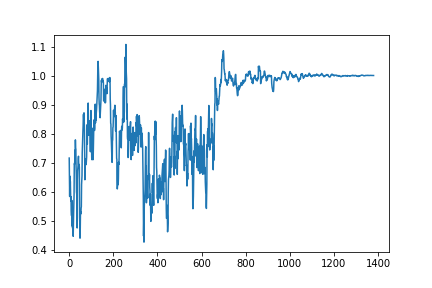
\includegraphics[width=\linewidth]{exp2_G_A.png}
        \caption{$\mathcal{L}_{G_A}$}
      \end{subfigure}
      \begin{subfigure}[b]{0.23\linewidth}
        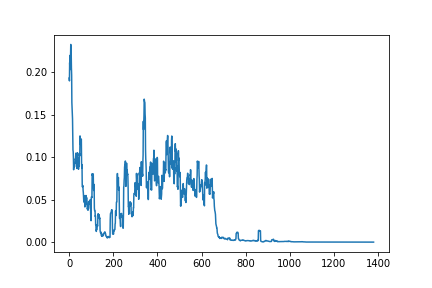
\includegraphics[width=\linewidth]{exp2_D_A.png}
        \caption{$\mathcal{L}_{D_A}$}
      \end{subfigure}
      \begin{subfigure}[b]{0.23\linewidth}
        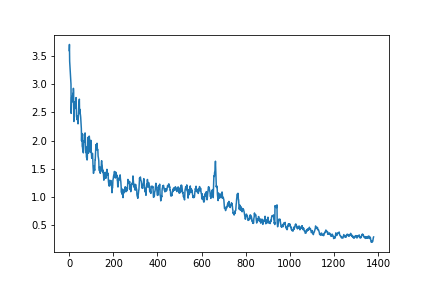
\includegraphics[width=\linewidth]{exp2_cycle_A.png}
        %\caption{$G_B(G_A(x))$}
        \caption{$\mathcal{L}_{cycle,A}$}
      \end{subfigure}
      \begin{subfigure}[b]{0.23\linewidth}
        \includegraphics[width=\linewidth]{exp2_idt_A.png}
        \caption{$\mathcal{L}_{iden,A}$}
      \end{subfigure}
      \begin{subfigure}[b]{0.23\linewidth}
        \includegraphics[width=\linewidth]{exp2_G_B.png}
        \caption{$\mathcal{L}_{G_B}$}
      \end{subfigure}
      \begin{subfigure}[b]{0.23\linewidth}
        \includegraphics[width=\linewidth]{exp2_D_B.png}
        \caption{$\mathcal{L}_{D_B}$}
      \end{subfigure}
      \begin{subfigure}[b]{0.23\linewidth}
        \includegraphics[width=\linewidth]{exp2_cycle_B.png}
        %\caption{$G_B(G_A(x))$}
        \caption{$\mathcal{L}_{cycle,B}$}
      \end{subfigure}
      \begin{subfigure}[b]{0.23\linewidth}
        \includegraphics[width=\linewidth]{exp2_idt_B.png}
        \caption{$\mathcal{L}_{iden,B}$}
      \end{subfigure}
      \caption{实验2 loss曲线}
      \label{fig:exp2loss}
\end{figure}

可以注意到图 \ref{fig:exp2loss} 中生成器在epoch96附近的$\mathcal{L}_{G_X}$突然崩坏
而分类器的$\mathcal{L}_{D_X}$的收敛于0,暗示着
$D_X$的过于强势。然而说到底$G_X$也一直在优化,它又在优化什么呢?可以看到重建损失$\mathcal{L}_{cycle}$与
恒等映射损失$\mathcal{L}_{iden}$作为生成器的目标之一一直在下降,只是在$\mathcal{L}_{G_X}$崩坏的同时,
有一个更快的下降的趋势,说明算法的最速方向被放到了这两个损失上,使得我们真正的目标反而无法得到优化,
这说明这两个损失的不恰当权重在上下文不恰当时反而使得算法效果更恶化。

\subsubsection{实验3}

epoch96附近到底发生了什么呢?我这只有日志和快照可以看到,所以我打算从epoch 90时的模型快照开始重新迭代看看这是不是必然的,
结果发现到模型不再陷入上文所述的困境中,最后效果图如图 \ref{fig:exp3epoch194} 所示,
loss如图 \ref{fig:exp3loss} 所示,并未观测到明显的崩坏现象, 看来这还是有一定随机性的。

\begin{figure}[htb]
    \centering
    \begin{subfigure}[b]{0.23\linewidth}
        \includegraphics[width=\linewidth]{exp3_epoch194_real_A.png}
        \caption{$x \in A$}
      \end{subfigure}
      \begin{subfigure}[b]{0.23\linewidth}
        \includegraphics[width=\linewidth]{exp3_epoch194_fake_B.png}
        \caption{$G_A(x)$}
      \end{subfigure}
      \begin{subfigure}[b]{0.23\linewidth}
        \includegraphics[width=\linewidth]{exp3_epoch194_rec_A.png}
        %\caption{$G_B(G_A(x))$}
        \caption{$G_{BA}(x))$}
      \end{subfigure}
      \begin{subfigure}[b]{0.23\linewidth}
        \includegraphics[width=\linewidth]{exp3_epoch194_idt_A.png}
        \caption{$G_A(y)$}
      \end{subfigure}
      \begin{subfigure}[b]{0.23\linewidth}
        \includegraphics[width=\linewidth]{exp3_epoch194_real_B.png}
        \caption{$y \in B$}
      \end{subfigure}
      \begin{subfigure}[b]{0.23\linewidth}
        \includegraphics[width=\linewidth]{exp3_epoch194_fake_A.png}
        \caption{$G_B(y)$}
      \end{subfigure}
      \begin{subfigure}[b]{0.23\linewidth}
        \includegraphics[width=\linewidth]{exp3_epoch194_rec_B.png}
        %\caption{$G_A(G_B(y))$}
        \caption{$G_{AB}(y))$}
      \end{subfigure}
      \begin{subfigure}[b]{0.23\linewidth}
        \includegraphics[width=\linewidth]{exp3_epoch194_idt_B.png}
        \caption{$G_B(x)$}
      \end{subfigure}
      \caption{实验3 epoch194的结果}
      \label{fig:exp3epoch194}
\end{figure}

\begin{figure}[htb]
    \centering
    \begin{subfigure}[b]{0.23\linewidth}
        \includegraphics[width=\linewidth]{exp3_G_A.png}
        \caption{$\mathcal{L}_{G_A}$}
      \end{subfigure}
      \begin{subfigure}[b]{0.23\linewidth}
        \includegraphics[width=\linewidth]{exp3_D_A.png}
        \caption{$\mathcal{L}_{D_A}$}
      \end{subfigure}
      \begin{subfigure}[b]{0.23\linewidth}
        \includegraphics[width=\linewidth]{exp3_cycle_A.png}
        %\caption{$G_B(G_A(x))$}
        \caption{$\mathcal{L}_{cycle,A}$}
      \end{subfigure}
      \begin{subfigure}[b]{0.23\linewidth}
        \includegraphics[width=\linewidth]{exp3_idt_A.png}
        \caption{$\mathcal{L}_{iden,A}$}
      \end{subfigure}
      \begin{subfigure}[b]{0.23\linewidth}
        \includegraphics[width=\linewidth]{exp3_G_B.png}
        \caption{$\mathcal{L}_{G_B}$}
      \end{subfigure}
      \begin{subfigure}[b]{0.23\linewidth}
        \includegraphics[width=\linewidth]{exp3_D_B.png}
        \caption{$\mathcal{L}_{D_B}$}
      \end{subfigure}
      \begin{subfigure}[b]{0.23\linewidth}
        \includegraphics[width=\linewidth]{exp3_cycle_B.png}
        %\caption{$G_B(G_A(x))$}
        \caption{$\mathcal{L}_{cycle,B}$}
      \end{subfigure}
      \begin{subfigure}[b]{0.23\linewidth}
        \includegraphics[width=\linewidth]{exp3_idt_B.png}
        \caption{$\mathcal{L}_{iden,B}$}
      \end{subfigure}
      \caption{实验3 loss曲线}
      \label{fig:exp3loss}
\end{figure}

\subsubsection{实验4}

这里将$\mathcal{L}_{iden}$的权重从$0.5$调到$1.0$从头迭代完200 epoch,
虽然根据之前结论当时应该做相反的调整看看是不是有改善才对,不过当时没画loss图。结果与实验3差不多。
所以只提供loss曲线图 与前面比较。

\begin{figure}[htb]
    \centering
    \begin{subfigure}[b]{0.23\linewidth}
        \includegraphics[width=\linewidth]{exp4_G_A.png}
        \caption{$\mathcal{L}_{G_A}$}
      \end{subfigure}
      \begin{subfigure}[b]{0.23\linewidth}
        \includegraphics[width=\linewidth]{exp4_D_A.png}
        \caption{$\mathcal{L}_{D_A}$}
      \end{subfigure}
      \begin{subfigure}[b]{0.23\linewidth}
        \includegraphics[width=\linewidth]{exp4_cycle_A.png}
        %\caption{$G_B(G_A(x))$}
        \caption{$\mathcal{L}_{cycle,A}$}
      \end{subfigure}
      \begin{subfigure}[b]{0.23\linewidth}
        \includegraphics[width=\linewidth]{exp4_idt_A.png}
        \caption{$\mathcal{L}_{iden,A}$}
      \end{subfigure}
      \begin{subfigure}[b]{0.23\linewidth}
        \includegraphics[width=\linewidth]{exp4_G_B.png}
        \caption{$\mathcal{L}_{G_B}$}
      \end{subfigure}
      \begin{subfigure}[b]{0.23\linewidth}
        \includegraphics[width=\linewidth]{exp4_D_B.png}
        \caption{$\mathcal{L}_{D_B}$}
      \end{subfigure}
      \begin{subfigure}[b]{0.23\linewidth}
        \includegraphics[width=\linewidth]{exp4_cycle_B.png}
        %\caption{$G_B(G_A(x))$}
        \caption{$\mathcal{L}_{cycle,B}$}
      \end{subfigure}
      \begin{subfigure}[b]{0.23\linewidth}
        \includegraphics[width=\linewidth]{exp4_idt_B.png}
        \caption{$\mathcal{L}_{iden,B}$}
      \end{subfigure}
      \caption{实验4 loss曲线}
      \label{fig:exp3loss}
\end{figure}

\subsubsection{实验5}

前面生成器用的resnet\_9blocks的实现有9个residual block,如果能用更小的网络结构可以得到相同的效果就可以加速训练和
测试了。所以我考虑了仅使用6个residual block的实现,即结构改为:
c7s1-64,d128,d256,R256x6,u128,u64,c7s1-3,迭代141 epoch。结果类似实验2的结果,生成效果见图 \ref{fig:exp5epoch140}
loss曲线图与实验6的loss曲线放在一张图中比较。

\begin{figure}[htb]
    \centering
    \begin{subfigure}[b]{0.23\linewidth}
        \includegraphics[width=\linewidth]{exp5_epoch140_real_A.png}
        \caption{$x \in A$}
      \end{subfigure}
      \begin{subfigure}[b]{0.23\linewidth}
        \includegraphics[width=\linewidth]{exp5_epoch140_fake_B.png}
        \caption{$G_A(x)$}
      \end{subfigure}
      \begin{subfigure}[b]{0.23\linewidth}
        \includegraphics[width=\linewidth]{exp5_epoch140_rec_A.png}
        %\caption{$G_B(G_A(x))$}
        \caption{$G_{BA}(x))$}
      \end{subfigure}
      \begin{subfigure}[b]{0.23\linewidth}
        \includegraphics[width=\linewidth]{exp5_epoch140_idt_A.png}
        \caption{$G_A(y)$}
      \end{subfigure}
      \begin{subfigure}[b]{0.23\linewidth}
        \includegraphics[width=\linewidth]{exp5_epoch140_real_B.png}
        \caption{$y \in B$}
      \end{subfigure}
      \begin{subfigure}[b]{0.23\linewidth}
        \includegraphics[width=\linewidth]{exp5_epoch140_fake_A.png}
        \caption{$G_B(y)$}
      \end{subfigure}
      \begin{subfigure}[b]{0.23\linewidth}
        \includegraphics[width=\linewidth]{exp5_epoch140_rec_B.png}
        %\caption{$G_A(G_B(y))$}
        \caption{$G_{AB}(y))$}
      \end{subfigure}
      \begin{subfigure}[b]{0.23\linewidth}
        \includegraphics[width=\linewidth]{exp5_epoch140_idt_B.png}
        \caption{$G_B(x)$}
      \end{subfigure}
      \caption{实验5 epoch140的结果}
      \label{fig:exp5epoch140}
\end{figure}

\subsubsection{实验6}

由于感觉生成器两个损失越俎代庖,所以给$\mathcal{L}_{GAN}$的损失权重加一倍迭代200轮。对比两者的损失曲线可见 
\ref{fig:exp6loss},虽然实验6的两个损失都比实验5的同时高,但效果却并没有多改善,也许这还是生成器与鉴别器相对能力
差距较大导致的。

\begin{figure}[htb]
    \centering
    \begin{subfigure}[b]{0.23\linewidth}
        \includegraphics[width=\linewidth]{exp6_G_A.png}
        \caption{$\mathcal{L}_{G_A}$}
      \end{subfigure}
      \begin{subfigure}[b]{0.23\linewidth}
        \includegraphics[width=\linewidth]{exp6_D_A.png}
        \caption{$\mathcal{L}_{D_A}$}
      \end{subfigure}
      \begin{subfigure}[b]{0.23\linewidth}
        \includegraphics[width=\linewidth]{exp6_cycle_A.png}
        %\caption{$G_B(G_A(x))$}
        \caption{$\mathcal{L}_{cycle,A}$}
      \end{subfigure}
      \begin{subfigure}[b]{0.23\linewidth}
        \includegraphics[width=\linewidth]{exp6_idt_A.png}
        \caption{$\mathcal{L}_{iden,A}$}
      \end{subfigure}
      \begin{subfigure}[b]{0.23\linewidth}
        \includegraphics[width=\linewidth]{exp6_G_B.png}
        \caption{$\mathcal{L}_{G_B}$}
      \end{subfigure}
      \begin{subfigure}[b]{0.23\linewidth}
        \includegraphics[width=\linewidth]{exp6_D_B.png}
        \caption{$\mathcal{L}_{D_B}$}
      \end{subfigure}
      \begin{subfigure}[b]{0.23\linewidth}
        \includegraphics[width=\linewidth]{exp6_cycle_B.png}
        %\caption{$G_B(G_A(x))$}
        \caption{$\mathcal{L}_{cycle,B}$}
      \end{subfigure}
      \begin{subfigure}[b]{0.23\linewidth}
        \includegraphics[width=\linewidth]{exp6_idt_B.png}
        \caption{$\mathcal{L}_{iden,B}$}
      \end{subfigure}
      \caption{实验5,6 loss曲线}
      \label{fig:exp6loss}
\end{figure}

\subsubsection{实验7}

之前的实验中均采取将两域图片压成同尺寸处理的方法,如果A域图片作为本来的大尺寸高分辨率的图片保持相对较多的信息
($192/times 192$,取$192$是因为注意到$48$放大4倍后为$192$
)而B域图片不进行蹩脚的升采样(保持$48\times 48$而非$64\times 64$),结果是否会有改善呢?直接
修改输入输出是不可行的,因为$\mathcal{L}_{iden}$要求两域相同,一种方式是直接取消这个项,不过我是直接线性插值。
而且此时两个生成器的结构是不一样的。$G_A$为c7s1-32,d64,d128,R128x6,c7s1-3。即去掉将尺寸增大(恢复)的层,同时
隐单元数全体除以2,由于显存的原因\footnote{这里也考虑过float16替换float32的优化,不过碰到一些奇怪的BUG就算了。}
而$G_B$类似,为:c7s1-32,R128x6,u128,u64,c7s1-3。即去掉了降尺寸的层,同时单元数减一半。而判别器与之前结构类似,
但单元数除以4以令两者的能力差不那么大以期能够改善优化。

虽然进行了一些优化,但是算法运行的很慢,我间间断断运行了3天才完成了61 epoch。效果也不怎么样,如图 
\ref{fig:exp7epoch61}所示。可能还是生成器能力不够的原因。

\begin{figure}[htb]
    \centering
    \begin{subfigure}[b]{0.23\linewidth}
        \includegraphics[width=\linewidth]{exp7_epoch061_real_A.png}
        \caption{$x \in A$}
      \end{subfigure}
      \begin{subfigure}[b]{0.23\linewidth}
        \includegraphics[width=\linewidth]{exp7_epoch061_fake_B.png}
        \caption{$G_A(x)$}
      \end{subfigure}
      \begin{subfigure}[b]{0.23\linewidth}
        \includegraphics[width=\linewidth]{exp7_epoch061_rec_A.png}
        %\caption{$G_B(G_A(x))$}
        \caption{$G_{BA}(x))$}
      \end{subfigure}
      \begin{subfigure}[b]{0.23\linewidth}
        \includegraphics[width=\linewidth]{exp7_epoch061_idt_A.png}
        \caption{$G_A(y)$}
      \end{subfigure}
      \begin{subfigure}[b]{0.23\linewidth}
        \includegraphics[width=\linewidth]{exp7_epoch061_real_B.png}
        \caption{$y \in B$}
      \end{subfigure}
      \begin{subfigure}[b]{0.23\linewidth}
        \includegraphics[width=\linewidth]{exp7_epoch061_fake_A.png}
        \caption{$G_B(y)$}
      \end{subfigure}
      \begin{subfigure}[b]{0.23\linewidth}
        \includegraphics[width=\linewidth]{exp7_epoch061_rec_B.png}
        %\caption{$G_A(G_B(y))$}
        \caption{$G_{AB}(y))$}
      \end{subfigure}
      \begin{subfigure}[b]{0.23\linewidth}
        \includegraphics[width=\linewidth]{exp7_epoch061_idt_B.png}
        \caption{$G_B(x)$}
      \end{subfigure}
      \caption{实验7 epoch61的结果}
      \label{fig:exp7epoch61}
\end{figure}

\section{结论}

由于时间受限,只做了三个微小的方法来从不同的方式来解决Sprite sheet自动生成的问题,虽然效果都不好,但还是学习了一个。
其中Delaunay三角分割映射可以考虑使用SIFT之类的自动寻找关键点,再运用关键点匹配算法匹配之,但考虑到这些算法甚至
在同一个域时都经常失败,在画风不同的两个域中无监督地匹配,不利用深度学习方法而依赖人工特征设计几乎是不可能的。
正态建模是我看特征脸以及SVM学到的特征地可视化时想到的,也是我感觉这些严重依赖固定位置,大小地分类器地用处所在,
尽管本身计算量小,但金字塔和滑动窗口可是想增加多少计算量就可以计算多少计算量。从而它在不同分布地图像中的推断
地失败也就是可以预料的了,正如正文中提到的,说到底它只不过是个蹩脚地考虑全二阶相关的方法,只相当于神经网络
的一层,叠加分层模型或者混合模型或者平滑也许可以缓解这个问题,但如果那样为什么不直接去用GAN和VAE?传统方法的悲剧。
CycleGAN的结果,正如原文\cite{zhu2017unpaired}提到的,在复杂的具有大形变的迁移常常失败,而我因为机能受限只能大大
削减了图片的尺寸,造成了模式坍缩的问题,从一些没公布的实验数据可以明显看到$G_B(y)$的结果往往就是少数几张原图。
而或者又削减隐单元基数,这使得网络能力下降,基本就只能拟合一些纹理,可以看到$G_A$就是给图涂上一些RPGMaker Sprite式
对比度明显的纹理,而$G_B$就是把Sprite加上一层光照,与之相对应的两个域尺寸不相同的实验花费太大,没有坐满200 epochs,
不过也可以猜到结果应该不怎么样。此外,Sprite Sheet真正核心的问题,用一个“素材”去产生12个或更多的变体并没有探索,
因为这些方法甚至在单个情况的生成都不怎么样,就不自取其辱了。总之Sprite Sheet生成这个有着明显的工业价值的问题
之所以一直没有人解决看来是有道理的,确实很有难度,我这短短的时间内也解决不了。

\bibliography{paper} 
\bibliographystyle{ieeetr}
%\bibliographystyle{apalike}


\end{document}